\documentclass[12pt]{article}
\usepackage{blindtext}
\usepackage[T1]{fontenc}
\usepackage[utf8]{inputenc}
\usepackage{amssymb} % for \smallsetminus
\usepackage{listings}
\usepackage{xcolor}
\usepackage{babel}
\usepackage{caption}
\usepackage{subcaption}
\usepackage{graphicx}



\title{DLVC 2020, Exercises 1}

\author{
  Dominik Schörkhuber\\
  \texttt{01027470}
  \and
  Thomas Kaufmann\\
  \texttt{1129115}
}


\date{\today}

\begin{document}
	\maketitle
	
\section*{Questions}

\subsection*{What is image classification?}

Image classification is the task of assigning labels to images or contents of images. 

\subsection*{What is the purpose of training, validation and test sets and why do we need all of them?}

In general, machine learning techniques perform some kind of function approximation in a multidimensional space of a given domain. By adapting the function approximators' parameters in order to minimize a loss function for given a set of samples, one tries to obtain a model that performs well on the provided samples, but more importantly is generally applicable in arbitrary samples in the given domain. Since learning, however, is always subject to a rather limited set of samples compared to the enormous size of the domain (e.g. $256 \times 256 \times 256^3$ for moderate 8-bit RGB images), imbalanced or biased training sets can easily lead to an overfitted model that performs well on the training set, but is not able to generalize on arbitrary samples. To this end, a common approach is to split samples into three independent sets, namely training, validation and test set. Tuning of model parameters (e.g. weight matrix) is performed on the training set, whereas hyper parameters, like learning rates, can be optimized based on the models performance on the validation set. Once both optimizations have converged or a time limit has been reached, the models performance can be validation with the independent training set. Alternatively to the described percentage split approach, often n-fold cross-validation techniques are applied. In \emph{deep learning}, however, where large models and vast parameter spaces are frequently encountered, computation time is a scarce resources, where extensive cross-validation techniques may become infeasible. 

\subsection*{How do linear classifiers work?}



\section*{Project Results}

\subsection*{Hyper Parameter Tuning}
Hyper parameter tuning was conduced with a random search over $300$ iterations in the parameter space induced by the learning rate $[0,1]$, the momentum $[0,1]$ and the momentum's type (classical and nesterov). Models performance was evaluated with its accuracy on the validation set. 
	
	
	
\begin{figure}
\centering
\begin{subfigure}{.8\textwidth}
  \centering
  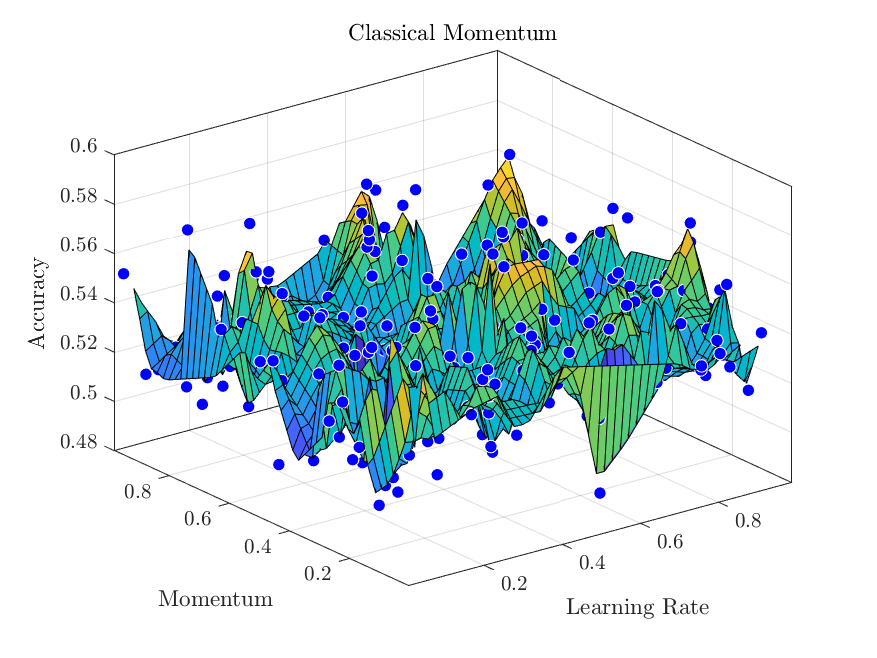
\includegraphics[width=.8\linewidth]{tuning-classical.pdf}
  \subcaption{}
  \label{fig:sub1}
\end{subfigure}

\begin{subfigure}{.8\textwidth}
  \centering
  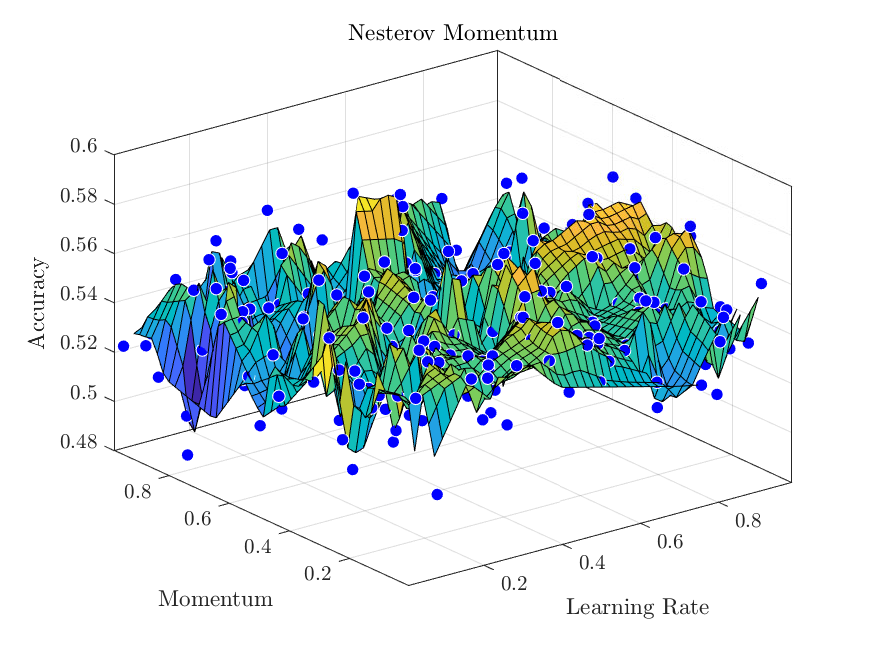
\includegraphics[width=.8\linewidth]{tuning-nesterov.pdf}
    \subcaption{}
  \label{fig:sub2}
\end{subfigure}
\caption{Hyper Parameter Space with classical (\ref{fig:sub1}) and Nesterov momentum (\ref{fig:sub2})}
\label{fig:test}
\end{figure}
	
	
	
\end{document}